\documentclass{article}
\usepackage[utf8]{inputenc}
\usepackage{subcaption}
\usepackage{amsmath}
\usepackage{amssymb}
\usepackage{hyperref}
\usepackage{titlesec}
\usepackage{xcolor}
\usepackage{fancyhdr}
\usepackage{listings}
\usepackage{graphicx}
\usepackage{multirow}
\usepackage[rightcaption]{sidecap}
\usepackage{verbatim}
\usepackage[backend=biber,style=numeric,sortcites,natbib=true,sorting=none]{biblatex}
\usepackage [ a4paper , hmargin =1.2 in , bottom =1.5 in ] { geometry }
\addbibresource{report.bib}
\usepackage{xcolor}
\definecolor{lightgray}{rgb}{0.95, 0.95, 0.95}
\definecolor{darkgray}{rgb}{0.4, 0.4, 0.4}
\definecolor{purple}{rgb}{0.65, 0.12, 0.82}
\definecolor{editorGray}{rgb}{0.95, 0.95, 0.95}
\definecolor{editorOcher}{rgb}{1, 0.5, 0} % #FF7F00 -> rgb(239, 169, 0)
\definecolor{editorGreen}{rgb}{0, 0.5, 0} % #007C00 -> rgb(0, 124, 0)
\definecolor{orange}{rgb}{1,0.45,0.13}		
\definecolor{olive}{rgb}{0.17,0.59,0.20}
\definecolor{brown}{rgb}{0.69,0.31,0.31}
\definecolor{purple}{rgb}{0.38,0.18,0.81}
\definecolor{lightblue}{rgb}{0.1,0.57,0.7}
\definecolor{lightred}{rgb}{1,0.4,0.5}
\definecolor{codegreen}{rgb}{0,0.6,0}
\definecolor{codegray}{rgb}{0.5,0.5,0.5}
\definecolor{codepurple}{rgb}{0.58,0,0.82}
\definecolor{backcolour}{rgb}{0.95,0.95,0.92}

\hypersetup{
    colorlinks=true,
    linkcolor=blue,
    filecolor=magenta,      
    urlcolor=cyan,
}

\lstdefinestyle{mystyle}{
    backgroundcolor=\color{backcolour},   
    commentstyle=\color{codegreen},
    keywordstyle=\color{magenta},
    numberstyle=\tiny\color{codegray},
    stringstyle=\color{codepurple},
    basicstyle=\ttfamily\footnotesize,
    breakatwhitespace=false,         
    breaklines=true,                 
    captionpos=b,                    
    keepspaces=true,                 
    numbers=left,                    
    numbersep=5pt,                  
    showspaces=false,                
    showstringspaces=false,
    showtabs=false,                  
    tabsize=2
}
%CSS 
\lstdefinelanguage{CSS}{
  keywords={margin:,padding:,display:,flex-direction:,justify-content:,align-items:,background-color:,height:,font-family:,margin-bottom:,text-shadow:,font-size:,position:,text-align:,border-radius:,box-shadow:,grid-template-columns:,grid-gap:,width:,align-content:,border:,cursor:,line-height:,transform:,pointer-events:,animation:,margin-right:,margin-top:,color:,top:,left:,right:,opacity:,transition:,z-index:,},	
  sensitive=true,
  morecomment=[l]{//},
  morecomment=[s]{/*}{*/},
  morestring=[b]',
  morestring=[b]",
  alsoletter={:},
  alsodigit={-}
}

% JavaScript
\lstdefinelanguage{JavaScript}{
  morekeywords={typeof, new, true, false, catch, function, return, null, catch, switch, var, if, in, while, do, else, case, break, let, const, event},
  morecomment=[s]{/*}{*/},
  morecomment=[l]//,
  morestring=[b]",
  morestring=[b]'
}

\lstset{style=mystyle}

\addbibresource{references.bib}

% Add header and footer code here
\pagestyle{fancy}
\fancyhead[R]{Sanskar Shaurya}
\fancyhead[L]{HTML Project}
\fancyfoot[C]{Page \thepage}
% You may also add path to the images optionally
\graphicspath{{./images/}}
\begin{document}

% preamble
\title{CS104 Course Project\protect\\ Minesweeper Cricket}
\author{Sanskar Shaurya}
\date{}
\maketitle

\tableofcontents
\clearpage

\section{Introduction}
In this project, I have created an exciting game that combines elements of Minesweeper and Cricket. The objective of the game is to click on blocks within a grid and accumulate runs while avoiding fielders. Let's dive into the details of the game and explore the additional customizations that have been implemented. The game begins with a grid of blocks, where each block represents a potential score or a fielder. The player's goal is to reveal blocks and accumulate as many runs as possible without encountering a fielder.


%code of section 2, make appr
\section{Customisations}
\subsection{Two Game Modes}
I have given the player the option to either play this game alone or with a friend, when the game starts the player has to choose which game mode he wants to play. The screen corresponding to this is:
\newline
\newline
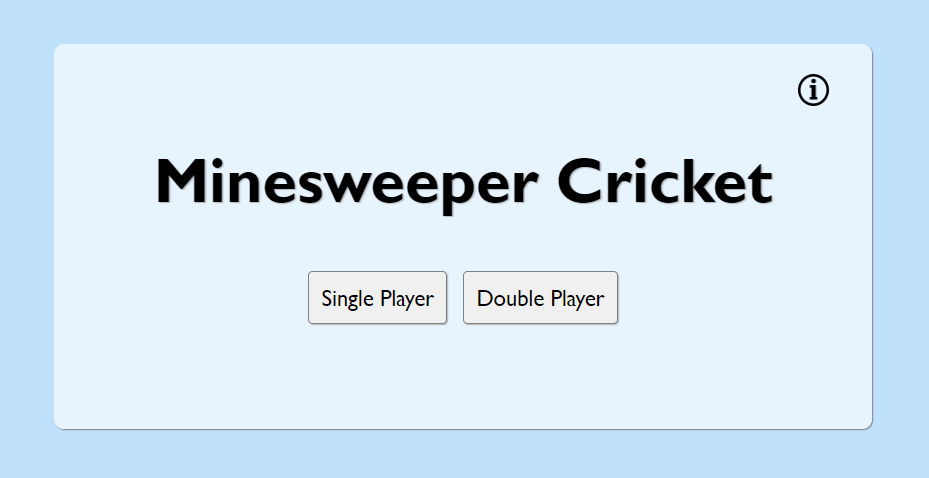
\includegraphics[width=\textwidth]{images/First Screen.png}
\newline
The mechanics of the two game modes are:
\begin{itemize}
    \item In the Single Player mode, the player has to score as many runs as he can before getting out
    \item In the Double Player mode, two players play this game turn-wise. The HTML asks for the names of both the players first and then starts the game. When the first player gets out, the second player continues playing till he gets out too. The player with the highest number of runs wins.
\end{itemize}
\subsection{Variable Grid Size}
Before starting the game in any of the two above modes, the player has to choose from one of the 5 different available grid sizes, ranging from 6 x 6 to 10 x 10. The game will then produce a grid of the appropriate dimension with fielders spread randomly throughout the "field" (grid). The number of fielders is dependent on the grid size, this is to make the game of smaller grid-sizes not get over very quickly.
\subsection{Variable Number of Runs}
Each block has a probability of getting one of the following runs allocated to it: 1, 2, 4, 6, or the shield power-up. I have modified these probabilities such that the chance of getting a boundary-score is less than that of a single or a double.
\subsection{Shield Power Up}
Each block also has a chance of containing the shield power-up. This power up when activated, will allow the player to not get out in the next three turns even if they click on a block with a fielder.
\newline
\begin{center}
    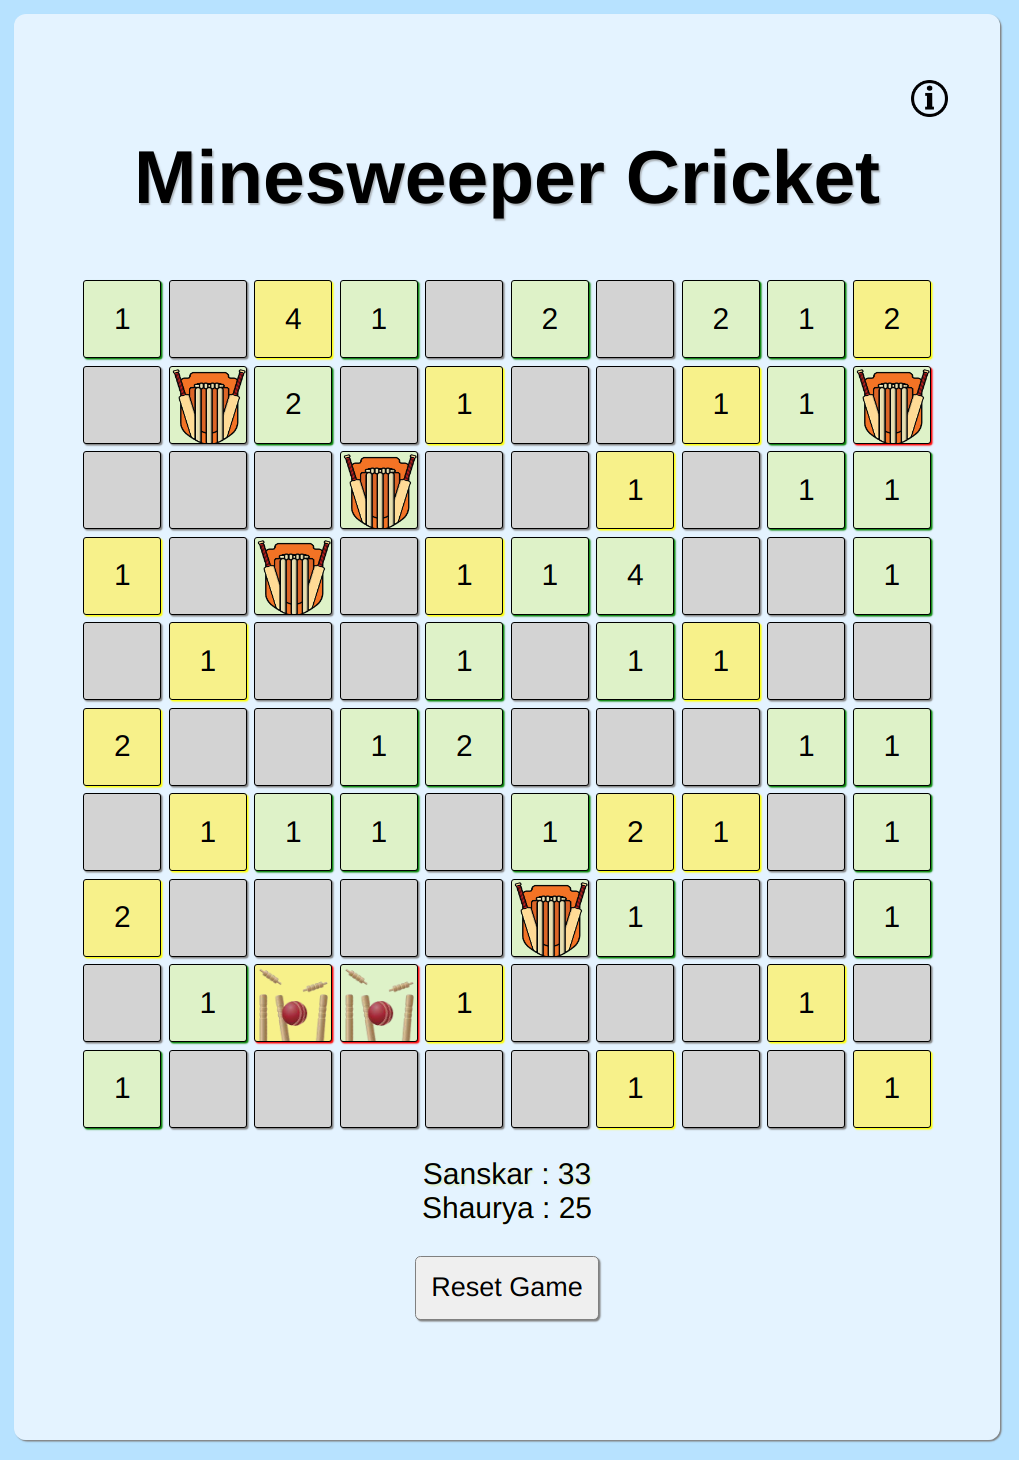
\includegraphics[scale = 0.33]{images/Game.png}
    \newline
    \newline
    An example of the game being played between two players showcasing some of the customisations
\end{center}
\section{Stylesheet}
\subsection{Colors}
I have used a combination of blue, light blue, gray, and white to make the webpage visually appealing. The elements also have a shadow which makes them pop on the screen. 
\subsection{Info and Back Button}
I have also added an info button which, when clicked, will open up an information box that takes up the entire screen. There also is a back button that will take the player back to the previous screen. (Note: This button is not available when the game gets started)
\subsection{Grid Style \autocite{ref1}}
The boxes, when clicked, also get colored corresponding to the player who is playing. Green for Player-1 and Yellow for Player-2 in double-player mode and just Green in single-player mode. When hovering on a block, the block gets highlighted and when it gets clicked, it undergoes a scale-up animation\autocite{ref2,ref3} which makes the game more visually appealing. I have also added some border-radius to the grid-blocks so that the blocks don't look very sharp.
\subsection{Font Used}
I have used the "Gill Sans" font for this website. The color of the font is either black or white, depending on the background on which the text is written. 
\section{The JavaScript \autocite{ref5}}
Brief explanations of some of the functions I used:
\begin{itemize}
    \item[--] \textbf{single() : }This function sets the \emph{playerChoice} variable to 1, which makes the game proceed with the single player mode. This function is called when the player clicks on the Single Player button. 
    \item[--] \textbf{double() : }This function sets the \emph{playerChoice} variable to 2, which makes the game proceed with the double player mode. This function is called when the player clicks on the Double Player button. 
    \item[--] \textbf{backButton.addEventListener('click') : }This function is for the back button, makes the screen go to the previous one.\autocite{ref4}
    \item[--] \textbf{showGameGrid(gridSize) : }This function is executed when the player clicks on one of the grid-size options, it sets the variable \emph{size} equal to the value clicked by the user and proceeds onto the next screen corresponding to the game-mode selected.
    \item[--] \textbf{startSingleGame(gridSize) : }This is the main function of the single-player mode, it contains of all the sub-functions required for this mode to work properly. It generates blocks and gives them scores or shield based on some probability. It has some sub-functions which are listed below:
    \begin{itemize}
        \item[--] \textbf{handleBlockClick(event) : }This function is the main working part of the single-player mode. This function is called whenever the player clicks on any of the grid-blocks. Based on what the block contains, this function gives the player some runs, gets them a shield or gets them out and calls the \emph{endGame()} function.
        \item[--] \textbf{endGame(score) : }This function is called when the player clicks on a fielder block, It gives an alert giving the final score of the player and makes the reset button visible.
    \end{itemize}
    \item[--] \textbf{nameForm.addEventListener('submit') : }This function is for when the user submits the name form in the double player mode. It sets the player-1 and player-2 name corresponding to the values written in the text-fields. 
    \item[--] \textbf{startDoubleGame(gridSize) : }This is the main function of the double-player mode, it contains of all the sub-functions required for this mode to work properly. It generates blocks and gives them scores or shield based on some probability. It has some sub-functions which are listed below:
    \begin{itemize}
        \item[--] \textbf{handleBlockClick(event) : }This function handles the clicking of blocks for the double-player-mode. This checks who the current player is and applies the game logic to that player. It calls the \emph{togglePlayer()} function to the change the current player and the \emph{endGame()} function when both the players get out.
        \item[--] \textbf{togglePlayer() : }This is a simple function which just checks who the current player is and then swaps to the next player.
        \item[--] \textbf{endGame() : }This function ends the game when both of the players get out and makes the reset button visible.
    \end{itemize}
    \item[--] \textbf{resetButton.addEventListener('click') : }This is the function for the reset button, this makes every score go back to the default value of 0. This also clears the grid and makes it empty.
    \item[--] \textbf{generateRandomPositions(gridSize, count) : }This is the function which generates random fielder positions. It returns a 2D array which has the row and column indices of the fielder positions as elements and there are a total of \emph{count} elements which we have used corresponding to the grid size.
\end{itemize}
\clearpage
\section{Source Code}
\subsection{HTML}
\lstinputlisting[language=HTML]{code/main.html}
\subsection{CSS}
\lstinputlisting[language=CSS]{code/style.css}
\subsection{JavaScript}
\lstinputlisting[language=JavaScript]{code/script.js}
\printbibliography
\end{document}
